\documentclass[10pt]{article}

% Packages and macros go here
\usepackage[T1]{fontenc}
\usepackage{lmodern}
\usepackage[utf8x]{inputenx}
\usepackage{microtype}
\usepackage{framed}
\usepackage{listings}
\usepackage{vmargin}
\usepackage{setspace}
\usepackage{mathrsfs, mathenv}
\usepackage{amsmath, amsthm, amssymb, amsfonts, amscd}
\usepackage{graphicx}
\usepackage{epstopdf}
\usepackage[svgnames]{xcolor}
\usepackage{hyperref}
\usepackage[capitalise]{cleveref}
\hypersetup{citecolor=blue, colorlinks=true, linkcolor=black}
\setlength{\parskip}{6pt}
\setlength\parindent{0pt}
\usepackage{subcaption}
\usepackage{bbm}
\usepackage{cite}
\usepackage{verbatim}
\usepackage{pgfplots}
\usepackage{tikz}
\usepackage{etoolbox}
\usepackage{color}
\usepackage{lipsum}
\usepackage{ifthen}
\usepackage[linesnumbered, ruled, vlined]{algorithm2e}
\crefname{algocf}{Algorithm}{Algorithms}
\usepackage{autonum}

\theoremstyle{plain}
\newtheorem{theorem}{Theorem}[section]
\newtheorem{corollary}[theorem]{Corollary}
\newtheorem{lemma}[theorem]{Lemma}
\newtheorem{proposition}[theorem]{Proposition}
\numberwithin{equation}{section}

\theoremstyle{definition}
\newtheorem{definition}[theorem]{Definition}

\theoremstyle{remark}
\newtheorem{remark}[theorem]{Remark}
\newtheorem{assumption}[theorem]{Assumption}
\newtheorem{example}[theorem]{Example}


\ifpdf
  \DeclareGraphicsExtensions{.eps,.pdf,.png,.jpg}
\else
  \DeclareGraphicsExtensions{.eps}
\fi

\usepackage{mathtools}
% basics

% tables
\usepackage{booktabs}

% plots
\usepackage{pgfplots}
\usepackage{tikz}
\usetikzlibrary{patterns,arrows,decorations.pathmorphing,backgrounds,positioning,fit,matrix}
\usepackage[labelfont=bf]{caption}
\setlength{\belowcaptionskip}{-5pt}
\usepackage{here}
\usepackage[font=normal]{subcaption}

% Prevent itemized lists from running into the left margin inside theorems and proofs
\usepackage{enumitem}
\setlist[itemize]{leftmargin=.5in}
\setlist[enumerate]{leftmargin=.5in,topsep=3pt,itemsep=3pt,label=(\roman*)}

% Add a serial/Oxford comma by default.
\newcommand{\creflastconjunction}{, and~}

% Sets running headers as well as PDF title and authors
% title and authors

\newcommand{\email}[1]{\href{#1}{#1}}
\newcommand{\TheTitle}{Probabilistic methods for elliptic partial differential equations} 
\newcommand{\TheAuthors}{A. Abdulle, G. Garegnani}
%\headers{Random time steps for quantifying chaotic numerical integration}{\TheAuthors}
\title{{\TheTitle}}
\newcommand*\samethanks[1][\value{footnote}]{\footnotemark[#1]}
\author{Assyr Abdulle\thanks{Institute of Mathematics, \'Ecole Polytechnique F\'ed\'erale de Lausanne (\email{\{assyr.abdulle, giacomo.garegnani\}@epfl.ch})}
	\and
	Giacomo Garegnani\samethanks}
\date{}

\usepackage{amsopn}
\DeclareMathOperator{\diag}{diag}
\DeclarePairedDelimiter{\ceil}{\left\lceil}{\right\rceil}
\DeclarePairedDelimiter{\floor}{\lfloor}{\rfloor}
\DeclarePairedDelimiter{\abs}{\lvert}{\rvert}
\DeclarePairedDelimiter{\norm}{\lVert}{\rVert}
\renewcommand{\phi}{\varphi}
\renewcommand{\theta}{\vartheta}
\renewcommand{\Pr}{\mathbb{P}}
\newcommand{\btilde}{\widetilde}
\newcommand{\bhat}{\widehat}
\newcommand{\eqtext}[1]{\ensuremath{\stackrel{#1}{=}}}
\newcommand{\leqtext}[1]{\ensuremath{\stackrel{#1}{\leq}}}
\newcommand{\iid}{\ensuremath{\stackrel{\text{i.i.d.}}{\sim}}}
\newcommand{\totext}[1]{\ensuremath{\stackrel{#1}{\to}}}
\newcommand{\rightarrowtext}[1]{\ensuremath{\stackrel{#1}{\longrightarrow}}}
\newcommand{\leftrightarrowtext}[1]{\ensuremath{\stackrel{#1}{\longleftrightarrow}}}
\newcommand{\pdv}[2]{\ensuremath\partial_{#2}#1}
\newcommand{\N}{\mathbb{N}}
\newcommand{\R}{\mathbb{R}}
\newcommand{\C}{\mathbb{C}}
\newcommand{\OO}{\mathcal{O}}
\newcommand{\epl}{\varepsilon}
\newcommand{\diffL}{\mathcal{L}}
\newcommand{\prior}{\mathcal{Q}}
\newcommand{\defeq}{\coloneqq}
\newcommand{\eqdef}{\eqqcolon}
\newcommand{\Var}{\operatorname{Var}}
\newcommand{\E}{\operatorname{\mathbb{E}}}
\newcommand{\MSE}{\operatorname{MSE}}
\newcommand{\trace}{\operatorname{tr}}
\newcommand{\MH}{\mathrm{MH}}
\newcommand{\ttt}{\texttt}
\newcommand{\Hell}{d_{\mathrm{H}}}
\newcommand{\sksum}{{\textstyle\sum}}
\newcommand{\dd}{\, \mathrm{d}}
\renewcommand{\d}{\mathrm{d}}
\definecolor{shade}{RGB}{100, 100, 100}
\definecolor{bordeaux}{RGB}{128, 0, 50}
\newcommand{\corr}[1]{{\color{red}#1}}
\newcommand{\Tau}{\tau}
\newcommand{\LL}{L}
\newcommand{\HH}{H}
\newcommand{\WW}{W}
\newcommand{\mbf}{\mathbf}
\newcommand{\bfs}{\boldsymbol}
\newcommand{\todo}{{\color{red} TO DO}}
\newcommand{\X}{\mathbb{X}}
\newcommand{\nablar}{\nabla_{\hat x}}
\newcommand{\eval}[1]{\bigr\rvert_{#1}}
\newcommand{\normm}[1]{\norm{#1}_a}
%\newcommand{\normm}[1]{{\left\vert\kern-0.25ex\left\vert\kern-0.25ex\left\vert #1 
%		\right\vert\kern-0.25ex\right\vert\kern-0.25ex\right\vert}}

\usepackage[usestackEOL]{stackengine}
\newcommand\fop[3][9pt]{\mathop{\ensurestackMath{\stackengine{#1}%
			{\displaystyle#2}{\scriptstyle#3}{U}{c}{F}{F}{L}}}\limits}
\newcommand\finf[2][9pt]{\fop[#1]{\inf}{#2}}
\newcommand\fsum[2][14pt]{\fop[#1]{\sum}{#2}}

\definecolor{leg1}{RGB}{0,114,189}
\definecolor{leg2}{RGB}{217,83,25}
\definecolor{leg3}{RGB}{237,177,32}
\definecolor{leg4}{RGB}{126,47,142}
\definecolor{leg5}{RGB}{119,172,48}

\definecolor{leg21}{RGB}{62,38,169}
\definecolor{leg22}{RGB}{46,135,247}
\definecolor{leg23}{RGB}{55,200,151}
\definecolor{leg24}{RGB}{254,195,56}


\ifpdf
\hypersetup{
	pdftitle={\TheTitle},
	pdfauthor={\TheAuthors}
}
\fi


\begin{document}
\maketitle	

\begin{abstract} 
\end{abstract}

\textbf{AMS subject classification.}

\textbf{Keywords.}

\section{Introduction}

\todo \cite{AbG18, KeH16, KSH18, CCC16, CGS17}

\begin{equation}\label{eq:ellipticEquation}
\begin{aligned}
	-\nabla \cdot (\kappa \nabla u) &= f, &&\text{in } D,\\
	u &= g, &&\text{on } \partial D.
\end{aligned}
\end{equation}

\textbf{important:} review of probabilistic methods for PDEs and ODEs. Have PDEs really been treated already? How? Inverse problems: what is the current state of things? Has anyone gone infinite dimensional?

\section{Random mesh probabilistic Finite Elements} 

Weak formulation: bilinear form $a\colon V\times V \to \R$ and a linear functional $F\colon V \to \R$ satisfying the usual continuity and coercivity constraints, look for $u \in V$ satisfying
\begin{equation}
	a(u, v) = F(v),	
\end{equation}
for all functions $v \in V$. Galerkin formulation: for $V_h \subset V$ such that $\dim V_h < \infty$, find $u_h \in V_h$ such that
\begin{equation}
	a(u_h, v_h) = f(v_h), \quad \forall v_h \in V_h,\\
\end{equation}
for all $v_h \in V_h$. Given a triangulation $\mathcal T_h$ of the domain $D$, we choose $V_h$ to be the space of linear finite elements, i.e., $V_h = X_h^1 \cap V$, where 
\begin{equation}
	X_h^1 = \{v_h \in C^0(\overline D) \colon v_h|_{K} \in \mathcal P_1, \; \text{for all } K \in \mathcal T_h\},
\end{equation}
and where $\mathcal P_1$ is the space of polynomials of degree at most one. The finite element space can be written then as $V_h = \mathrm{span}\{\phi_i\}_{i=1}^N$, where the basis $\{\phi_i\}_{i=1}^N$ are the Lagrange basis functions. Hence, each $v_h \in V_h$ can be written as $v_h = \sum_{i=1}^N v_i \phi_i$, where $v_i$ are the coefficients of $v_h$ on the basis $\{\phi_i\}_{i=1}^N$. Our probabilistic method is based on a randomly perturbed mesh $\btilde {\mathcal T}_h$ which is defined as follows.

\begin{definition} \label{def:RandomMesh} Let us consider a domain $D \subset \R^d$ and a triangulation $\mathcal T_h$ characterised by the maximum diameter $h > 0$ of its elements and by the set of vertices $\mathcal N_h = \{x_i\}_{i=1}^{N}$ such that $\mathcal N_h = \mathcal N_h^I \cup \mathcal N_h^B$, where $\mathcal N_h^I$ and $\mathcal N_h^B$ are the vertices in the interior of $D$ and on $\partial D$ respectively, and where we denote $N_I = \abs{\mathcal N_h^I}$ and $N_B = \abs{\mathcal N_h^B}$. Given a probability space $(\Omega, \Sigma, \mu)$, the random mesh $\btilde {\mathcal T}_h$ is defined by a sequence of random variables $\{\alpha_i\}_{i=1}^{N_I}$, $\alpha_i \colon \Omega \to \R^d$, which are used to perturb the internal nodes as
	\begin{equation}
	\tilde x_i = x_i + \bar h_i^p \alpha_i, \; x_i \in \mathcal N_h^I
	\end{equation}
	where $p \geq 1$ and $\bar h_i$ is defined as the minimum diameter of the elements $K$ having $x_i$ as a vertex, i.e.
	\begin{equation}
	\bar h_i = \min_{K \in \Delta(x_i)} h_K,
	\end{equation}
	where $\Delta(x_i)$ is such set of elements. The vertices laying on $\partial D$ in $\mathcal T_h$ are unperturbed in $\btilde {\mathcal T}_h$.
\end{definition}

Once the perturbed mesh $\btilde {\mathcal T}_h$ is obtained, let us denote by $\btilde V_h$ the piecewise linear finite element space defined on $\btilde {\mathcal T}_h$. Let us remark that the space $\btilde V_h = \btilde V_h(\omega)$ is random itself, i.e., for each realisation of the random variables $\{\alpha_i\}_{i=1}^{N_I}$ we obtain a different perturbed finite element space.


\begin{definition} \label{def:ProbSolution} With the notation above, the probabilistic solution $\tilde u_h \colon \Omega \times D \to \R$ is a random field satisfying for all $\omega \in \Omega$
	\begin{equation}
		\tilde u_h(\omega, \cdot) \in \btilde V_h(\omega), \; \text{s.t. } a(\tilde u_h(\omega, \cdot), \tilde v_h) = F(\tilde v_h), \; \text{for all } \tilde v_h \in \btilde V_h(\omega). 
	\end{equation}
\end{definition}

Let us finally introduce the following assumption on the random variables defining the mesh perturbation. 
\begin{assumption} \label{as:MeshPerturbation}  The random variables $\alpha_i$ are chosen such that the perturbed mesh $\btilde {\mathcal T}_h$ has the same topology of the mesh $\mathcal T_h$ (e.g., no exchange of vertices in one-dimension and no crossing edges in two-dimensions) almost surely.  
\end{assumption}

\section{A priori error analysis}

Close finite element spaces, sum space \cite{GaL15, BaK93}. \corr{Introduce the main ideas.}

\begin{definition} Given two possibly disjoint linear finite element spaces $V_h$ and $\btilde V_h$, we denote by $V_h^+ = V_h + \btilde V_h$  the space of functions that can be written as the sum of a function in $V_h$ and a function in $\btilde V_h$, i.e., for any function $v_h^+ \in V_h^+$ there exists functions $v_h \in V_h$ and $\tilde v_h \in \btilde V_h$ such that $v_h^+ = v_h + \tilde v_h$. 
\end{definition}

\begin{remark} Clearly from the definition, we have the inclusion $(V_h \cup \btilde V_h) \subseteq V_h^+$. Moreover, with homogeneous boundary conditions $V_h \cap \btilde V_h = \{0\}$ almost surely. Hence, $V_h^+ = V_h \oplus \btilde V_h$ and the decomposition of $v_h^+ \in V_h^+$ is unique.
\end{remark}

\begin{lemma}\label{lem:ConvergenceGeneral} The solutions $u_h \in V_h$ and $\tilde u_h \in \btilde V_h$ satisfy almost surely in $\Omega$
	\begin{equation}
	\begin{aligned}
		\norm{u_h - \tilde u_h}_V^2 \leq \Bigl(\frac{M}{\alpha}\Bigr)^2 \finf{v_h, w_h \in V_h} \biggl(\finf{\tilde v_h, \tilde w_h \in \btilde V_h} \Bigl(&\norm{u_h^+ - w_h}_V \norm{\tilde u_h - v_h}_V + \\ 
		&\norm{u_h^+ - \tilde w_h}_V \norm{u_h - \tilde v_h}_V \Bigr)\biggr),
	\end{aligned}
	\end{equation}
	where $u_h^+ \in V_h^+$ is the solution of 
	\begin{equation}\label{eq:uHPlus}
		a(u_h^+ , v_h^+) = F(v_h^+),	
	\end{equation}
	for all $v_h^+ \in V_h^+$.
\end{lemma}
\begin{proof} Since $V_h$ and $\btilde V_h$ are both subspaces of $V_h^+$, we have
	\begin{equation}\label{eq:orthogonality}
	\begin{aligned}
		a(u_h^+ - u_h, v_h) &=0, \quad \forall v_h \in V_h,\\
		a(u_h^+ - \tilde u_h, \tilde v_h) &= 0, \quad \forall \tilde v_h \in \btilde V_h,
	\end{aligned}
	\end{equation}
	which means that $u_h$ and $\tilde u_h$ are the elliptic projection of $u_h^+$ onto $V_h$ and $\btilde V_h$ respectively. Hence, thanks to Cea's lemma
	\begin{equation}
	\begin{aligned}
		\norm{u_h^+ - u_h}_V \leq \frac{M}{\alpha}\norm{u_h^+ - w_h}_V,\\
		\norm{u_h^+ - \tilde u_h}_V \leq \frac{M}{\alpha}\norm{u_h^+ - \tilde w_h}_V,
	\end{aligned}
	\end{equation}
	for all $w_h \in V_h$ and $\tilde w_h \in \btilde V_h$.	Using the coercivity on $V$ of $a(\cdot, \cdot)$, adding and subtracting $a(u_h^+, u_h - \tilde u_h)$ and thanks to the orthogonality property \eqref{eq:orthogonality} we have for all $v_h \in V_h$ and $\tilde v_h \in \btilde V_h$
	\begin{equation}
	\begin{aligned}
		\alpha \norm{u_h - \tilde u_h}_V^2 &\leq a(u_h - \tilde u_h, u_h - \tilde u_h)\\
		&= a(u_h - u_h^+, u_h - \tilde u_h) + a(u_h^+ - \tilde u_h, u_h - \tilde u_h)\\
		&= a(u_h - u_h^+, v_h - \tilde u_h) + a(u_h^+ - \tilde u_h, u_h - \tilde v_h).
	\end{aligned}
	\end{equation}
	Thanks to the continuity of the bilinear form we then have for all $w_h \in V_h$ and $\tilde w_h \in \btilde V_h$ 
	\begin{equation}
	\begin{aligned}
		\alpha \norm{u_h - \tilde u_h}_V^2 &\leq M \Big(\norm{u_h^+ - u_h}_V\norm{\tilde u_h - v_h}_V + \norm{u_h^+ - \tilde u_h}_V\norm{u_h - \tilde v_h}_V\Big)\\
		&\leq \frac{M^2}{\alpha} \Big(\norm{u_h^+ - w_h}_V\norm{\tilde u_h - v_h}_V + \norm{u_h^+ - \tilde w_h}_V\norm{u_h - \tilde v_h}_V\Big),
	\end{aligned}
	\end{equation}
	which implies the result taking the infimum at the right hand side.
\end{proof}

Let us remark that the lemma above is valid for any choice of $V_h$ and $\btilde V_h$. In order to study the approximation of a function $v_h$ of $V_h$ with functions of $\btilde V_h$, we exploit the Legendre interpolation.

\begin{definition} We denote by $\Pi_h\colon V \to V_h$ and $\btilde \Pi_h\colon V \to \btilde V_h$ the Legendre piecewise linear interpolation operators on $V_h$ and $\btilde V_h$ respectively, i.e.,
	\begin{equation}
	\begin{aligned}
		\Pi_h v(x) = \fsum{x_j \in \mathcal N_h^I} v(x_j) \phi_j(x),\\
		\btilde \Pi_h v(x) = \fsum{\tilde x_j \in \btilde {\mathcal N}_h^I} v(x_j) \tilde \phi_j(x),
	\end{aligned}
	\end{equation}
	where $\{\phi_i\}_{i=1}^{N^I}$ and $\{\tilde \phi_i\}_{i=1}^{N^I}$ are the basis functions of $V_h$ and $\btilde V_h$ respectively.
\end{definition}

In the following lemma we characterise the Legendre interpolant $\btilde V_h$ through its values on the internal nodes of the original mesh $\mathcal T_h$.  

\begin{lemma}\label{lem:InterpPreliminary} Let $V_h$ and $\btilde V_h$ be defined as in \cref{def:RandomMesh}. Then for all $v_h \in V_h$ and all $x_i \in \mathcal N_h^I$ it holds
	\begin{equation}
		\btilde \Pi_h v_h(x_i) - v_h(x_i) = \bar h_i^p \alpha_i^\top \Big(\nabla v_h(\tilde x_i) - \nabla \btilde \Pi_h v_h(x_i)\Big).
	\end{equation}
\end{lemma}
\begin{proof} Let us denote $e_h = \btilde \Pi_h v_h - v_h$. An exact Taylor expansion of the linear basis function $\tilde \phi_j$ gives
\begin{equation}
\begin{aligned}
	e_h(x_i) &= \sum_{j} v_h(\tilde x_j) \phi_j(x_i) - v_h(x_i) \\
	&= \sum_j v_h(\tilde x_j) \Big(\tilde \phi_j(\tilde x_i) - \bar h_i^p \alpha_i^\top \nabla \tilde \phi_j(x_i)\Big) - v_h(x_i) \\
	&= v_h(\tilde x_i) - v_h(x_i) - \sum_j \bar h_i^p \alpha_i^\top v_h(\tilde x_j) \nabla \tilde \phi_j(x_i).
\end{aligned}
\end{equation}
We can now expand the function $v_h$, which is linear on the segment connecting $x_i$ and $\tilde x_i$, as
\begin{equation}\label{eq:TaylorVh}
	v_h(\tilde x_i) = v_h(x_i) + \bar h_i^p \alpha_i^\top \nabla v_h(\tilde x_i),
\end{equation}
to obtain
\begin{equation}
\begin{aligned}
	e_h(x_i) &= \bar h_i^p \alpha_i^\top \nabla v_h(\tilde x_i) - \bar h_i^p \alpha_i^\top \sum_j v_h(\tilde x_j) \nabla \tilde \phi_j(x_i) \\
	&= \bar h_i^p \alpha_i^\top \Big(\nabla v_h(\tilde x_i) - \nabla \btilde \Pi_h v_h(x_i)\Big),
\end{aligned}
\end{equation}
which is the desired result.
\end{proof}

Let us remark that the quality of the approximation given by the operator $\btilde \Pi_h$ depends on the regularity of $v_h$, as it will be clarified in the following. In order to exploit \cref{lem:ConvergenceGeneral}, it is necessary to control the interpolation of a function in $V_h^+$ on both $V_h$ and $\btilde V_h$, which is explained in the following lemma.

\begin{lemma}\label{lem:InterpSum} For all $v_h^+ \in V_h^+$ it holds
	\begin{equation}
	\begin{aligned}
		\Pi_h v_h^+ - v_h^+ &= \Pi_h \tilde v_h - \tilde v_h,  \\
		\btilde \Pi_h v^+_h - v_h^+ &= \Pi_h v_h - v_h,
	\end{aligned}
	\end{equation} 
	where $v_h \in V_h$ and $\tilde v_h \in \btilde V_h$ are the components of $v_h^+$ in $V_h$ and $\btilde V_h$ respectively, i.e., $v_h^+ = v_h + \tilde v_h$.
\end{lemma}
\begin{proof} The result can be obtained directly as $\Pi_h v_h = v_h$ for all $v_h \in V_h$ and $\btilde \Pi_h \tilde v_h = \tilde v_h$ for all $\tilde v_h \in \btilde V_h$.
\end{proof}

Let us now introduce the smoothness assumption we impose on the solution, which will constitute the framework for our analysis. 

\begin{assumption}\label{as:regularity} The exact solution $u$ of \eqref{eq:ellipticEquation} is in $\WW^{2, \infty}(D)$.
\end{assumption}

Under this assumption, the following result of uniform convergence holds.

\begin{theorem}[Theorem 3.3.7 of \cite{Cia02}]\label{thm:CiarletUniform} Under \cref{as:regularity}, the Finite Element solution $u_h \in V_h$ satisfies
	\begin{equation}\label{eq:W1InfErr}
	\begin{aligned}
		&\norm{u - u_h}_{\LL^\infty(D)} \leq C h^2 \abs{\log h}^{3/2} \abs{u}_{\WW^{2, \infty}(D)}, \\
		&\abs{u - u_h}_{\WW^{1, \infty}(D)} \leq C h \abs{\log h} \abs{u}_{\WW^{2, \infty}(D)},
	\end{aligned}
	\end{equation}
	where $C > 0$ is a constant independent of $h$.
\end{theorem}

\subsection{One-dimensional case}

\begin{lemma}\label{lem:Interp1D} Let $D = (0,1)$, $V_h$ be the finite element space defined on the regular grid $\{x_i = ih\}_{i=0}^{N}$ for $h = N^{-1}$ and $v_h \in V_h$. If there exists $v \in \WW^{2, \infty}(D)$ such that
	\begin{equation}\label{eq:RegularityInterp1D}
		\norm{v - v_h}_{\WW^{1, \infty}(D)} \leq C h \abs{\log h} \abs{v}_{\WW^{2, \infty}(D)},
	\end{equation} 
	then almost surely in $\Omega$
	\begin{equation}
	\begin{aligned}
		\norm{v_h - \btilde \Pi_h v_h}_{\LL^\infty(D)} &\leq Ch^{p+1} \abs{\log h},\\
		\abs{v_h - \btilde \Pi_h v_h}_{\HH^1(D)} &\leq Ch^{(p+1)/2} \abs{\log h},
	\end{aligned}
	\end{equation}
	where $C > 0$ is a constant independent of $h$. 
\end{lemma}
\begin{proof} Let us denote $e_h = \btilde \Pi_h v_h - v_h$. By definition $e_h(\tilde x_i) = 0$ for all $i = 0, \ldots, N$ and thanks to \cref{lem:InterpPreliminary}, in this setting
	\begin{equation}\label{eq:OneDNodes}
		e_h(x_i) = h^p \alpha_i \big(v_h'(\tilde x_i) - (\btilde \Pi_hv_h)'(x_i)\big).
	\end{equation}
	In the following, we denote by $\epl_i$ the quantity
	\begin{equation}
		\epl_i = v_h'(\tilde x_i) - (\btilde \Pi_hv_h)'(x_i).
	\end{equation}
	Before proceeding to the actual estimation of the error, we shall now bound $\abs{\epl_i}$. Let us consider without loss of generality $\alpha_i > 0$. In this case, it is clear that 
	\begin{equation}
		\epl_i = v_h'\eval{K_{i+1}} - (\btilde \Pi_hv_h)'\eval{\btilde K_i}.
	\end{equation}
	Let us decompose $\epl_i$ in two terms $\epl_{i, 1}$ and $\epl_{i, 2}$, defined as
	\begin{equation}
	\begin{aligned}
		\epl_{i, 1} &= v_h'\eval{K_{i+1}} - v_h'\eval{K_i}, \\
		\epl_{i, 2} &= v_h'\eval{K_i} - (\btilde \Pi_hv_h)'\eval{\btilde K_i},
	\end{aligned}	
	\end{equation}
	so that $\abs{\epl_i} \leq \abs{\epl_{i, 1}} + \abs{\epl_{i, 2}}$. Thanks to \eqref{eq:RegularityInterp1D} we have
	\begin{equation}\label{eq:gradDiffSmooth1d}
	\begin{aligned}
		\abs{\epl_{i, 1}} &\leq 2 \abs{v_h - v}_{\WW^{1,\infty}(D)} + \abs{v'(\bar x_i) - v'(\bar x_{i+1})}\\
		&\leq C h \abs{\log h} \abs{v}_{\WW^{2, \infty}(D)},
	\end{aligned}
	\end{equation}
	where we denote by $\bar x_j$ the midpoint of element $K_j$. Let us now consider $\epl_{i, 2}$. First, thanks to \eqref{eq:TaylorVh} and as we assumed $\alpha_i > 0$
	\begin{equation}
	\begin{aligned}
		(\btilde \Pi_hv_h)'\eval{\btilde K_i} &= \frac{1}{h + (\alpha_i - \alpha_{i-1})h^p} \big(v_h(\tilde x_i) - v_h(\tilde x_{i-1})\big) \\
		&= \frac{1}{h + (\alpha_i  - \alpha_{i-1})h^p} \Big(v_h(x_i) - v_h(x_{i-1}) + \big(\alpha_i v_h'(\tilde x_i) - \alpha_{i-1} v_h'(\tilde x_{i-1}) \big)h^p\Big)\\
		&= \frac{1}{1 + (\alpha_i - \alpha_{i-1})h^{p-1}} \Big(v_h'\eval{K_i} + \big(\alpha_i v_h'\eval{K_{i+1}} - \alpha_{i-1} v_h'(\tilde x_{i-1}) \big) h^{p-1} \Big),
	\end{aligned}
	\end{equation}
	where $v_h'(\tilde x_{i-1})$ could alternatively be equal to the derivative of $v_h$ on $K_{i-1}$ or $K_i$ depending on the sign of $\alpha_{i-1}$.	Let us now remark that
	\begin{equation}
		\frac{1}{1 + (\alpha_i - \alpha_{i-1})h^{p-1}} = 1 + R,
	\end{equation}
	where
	\begin{equation}
		R = \sum_{k=1}^\infty (-1)^k(\alpha_i - \alpha_{i-1})^k h^{k(p-1)},
	\end{equation}
	which implies
	\begin{equation}
	\begin{aligned}
		(\btilde \Pi_hv_h)'\eval{\btilde K_i} = v_h'\eval{K_i} &+ \big(\alpha_i v_h'\eval{K_{i+1}} - \alpha_{i-1} v_h'(\tilde x_{i-1}) \big) h^{p-1} \\
		&+ R \Big(v_h'\eval{K_i} + \big(\alpha_i v_h'\eval{K_{i+1}} - \alpha_{i-1} v_h'(\tilde x_{i-1}) \big)h^{p-1}\Big),
	\end{aligned}
	\end{equation}
	and finally
	\begin{equation}
	\begin{aligned}
		\abs{\epl_{i,2}} = \Bigl|&\big(\alpha_i v_h'\eval{K_{i+1}} - \alpha_{i-1} v_h'(\tilde x_{i-1}) \big) h^{p-1} \\
		&+ R \Big(v_h'\eval{K_i} + \big(\alpha_i v_h'\eval{K_{i+1}} - \alpha_{i-1} v_h'(\tilde x_{i-1}) \big)h^{p-1}\Big) \Bigr|.
	\end{aligned}
	\end{equation}
	Let us rewrite the expression above regrouping the terms by powers of $h$ as
	\begin{equation}
	\begin{aligned}
		\abs{\epl_{i,2}} &= \abs{\sum_{k=1}^{\infty} (-1)^k(\alpha_i - \alpha_{i-1})^{k-1}\Big((\alpha_i - \alpha_{i-1}) v_h'\eval{K_i} - \big(\alpha_i v_h'\eval{K_{i+1}} - \alpha_{i-1} v_h'(\tilde x_{i-1}) \big)\Big) h^{k(p-1)}}\\
		&= \abs{\sum_{k=1}^{\infty} (-1)^k(\alpha_i - \alpha_{i-1})^{k-1}\Big(\alpha_i \big(v_h'\eval{K_i} - v_h'\eval{K_{i+1}}\big) + \alpha_{i-1}\big(v_h'(\tilde x_{i-1}) - v_h'\eval{K_i}\big) \Big) h^{k(p-1)}} \\
		&\leq \sum_{k=1}^{\infty} \abs{\alpha_i - \alpha_{i-1}}^{k-1}\Big(\abs{\alpha_i}\abs{v_h'\eval{K_i} - v_h'\eval{K_{i+1}}} + \abs{\alpha_{i-1}} \abs{v_h'\eval{K_i} - v_h'(\tilde x_{i-1})} \Big) h^{k(p-1)}.
	\end{aligned}
	\end{equation}
	Hence, thanks to \eqref{eq:gradDiffSmooth1d} and to the hypotheses on the coefficients $\alpha_j$, we have
	\begin{equation}
		\abs{\epl_{i,2}} \leq C h^p \abs{\log h} \abs{v}_{\WW^{2, \infty}(D)},
	\end{equation} 
	which finally implies $\abs{\epl_i} \leq C h \abs{\log h}$ as $p\geq 1$. This means that the interpolation error satisfies on the nodes of the original mesh 
	\begin{equation}
		\abs{e_h(x_i)} \leq C h^{p+1} \abs{\log h} \abs{v}_{\WW^{2, \infty}(D)},
	\end{equation}
	and on the nodes of the perturbed mesh by definition $e_h(\tilde x_i) = 0$. We can now proceed to the estimation of the error. Let us now remark that since $e_h \in V_h^+$, the maximum of $e_h$ has to be realised on one of the nodes of the original mesh. Hence
	\begin{equation}
		\norm{e_h}_{\LL^{\infty}(D)} = \max_{x_i \in \mathcal N_h^{I}} \abs{e_h(x_i)} \leq C h^{p+1} \abs{\log h} \abs{v}_{\WW^{2, \infty}(D)},
	\end{equation}
	which implies the desired result for all $\LL^q$ spaces with $1 \leq q < \infty$.
%	Let us consider a single element of the modified grid $\btilde K_i = (\tilde x_{i-1}, \tilde x_i)$ and the $\LL^2$ norm. There are four distinct cases depending on the sign of the random variables $\alpha_{i-1}$ and $\alpha_i$. First, if $\alpha_{i-1} > 0$ and $\alpha_i < 0$, i.e., $\btilde K_i \subset K_i$, $e_h \equiv 0$ and we have trivially 
%	\begin{equation}
%		\norm{e_h}_{\LL^2(\btilde K_i)} = 0.
%	\end{equation}
%	The second and third cases are given by $\alpha_{i-1}$ and $\alpha_i$ having the same sign. Let us consider without loss of generality $\alpha_{i-1} < 0$ and $\alpha_i < 0$, i.e., $\tilde x_{i-1} < x_{i-1} < \tilde x_i < x_i$ and estimate the error in the $\LL^2$ norm. We separate the integral over the element as
%	\begin{equation}\label{eq:OneDDecomp1}
%		\int_{\btilde K_i} e_h^2 = \int_{\tilde x_{i-1}}^{x_{i-1}} e_h^2 + \int_{x_{i-1}}^{\tilde x_i} e_h^2.
%	\end{equation}
%	For the first integral, since $e_h(\tilde x_{i-1}) = 0$ and thanks to \eqref{eq:OneDNodes} we have
%	\begin{equation}
%		\int_{\tilde x_{i-1}}^{x_{i-1}} e_h^2 = \frac{\abs{\alpha_{i-1}}^3}{3} h^{3p} \epl_{i-1}^2.
%	\end{equation}
%	For the second interval, we get analogously
%	\begin{equation}
%		\int_{x_{i-1}}^{\tilde x_i} e_h^2 = \frac{\alpha_{i-1}^2(1 + \alpha_i h^{p-1})}{3}h^{2p+1}  \epl_{i-1}^2.
%	\end{equation}
%	Hence, thanks to \cref{as:MeshPerturbation} and to the estimate of $\abs{\epl_i}$ there exists a constant $C > 0$ 
%	\begin{equation}
%		\norm{e_h}_{\LL^2(\btilde K_i)}^2 \leq Ch^{2p+3} \abs{\log h}^2.
%	\end{equation}
%	Let us now consider the case $K_i \subset \btilde K_i$, i.e.,
%	\begin{equation}
%		\int_{\btilde K_i} e_h^2 = \int_{\tilde x_{i-1}}^{x_{i-1}} e_h^2 + \int_{x_{i-1}}^{x_i} e_h^2 + \int_{x_i}^{\tilde x_i} e_h^2.
%	\end{equation}
%	It is possible to compute the three integrals explicitly, thus getting
%	\begin{equation}
%	\begin{aligned}
%		\norm{e_h}_{\LL^2(\btilde K_i)}^2 &= \frac{1}{3}h^{3p}\big(\alpha_i^3 \epl_i^3 - \alpha_{i-1}^3\epl_{i-1}^2\big) + \frac{h^{2p+1}}{3}\big(\alpha_{i-1}^2\epl_{i-1}^2 + \alpha_i^2\epl_i^2 + \alpha_{i-1}\epl_{i-1} \alpha_i\epl_i\big)\\
%		&\leq Ch^{2p+3} \abs{\log h}^3.
%	\end{aligned}
%	\end{equation}
%%	Summing over the elements we get $\norm{e_h}_{\LL^2(D)} \leq Ch^{p+1} \abs{\log h}^{3/2}$, which is the desired result. 
	Let us now consider the $\HH^1$ semi-norm. We fix a single element of the modified grid $\btilde K_i = (\tilde x_{i-1}, \tilde x_i)$. There are four distinct cases depending on the sign of the random variables $\alpha_{i-1}$ and $\alpha_i$. First, if $\alpha_{i-1} > 0$ and $\alpha_i < 0$, i.e., $\btilde K_i \subset K_i$, $e_h \equiv 0$ and we have trivially $\abs{e_h}_{\HH^1(\tilde K)} = 0$. We now fix $\alpha_{i-1} < 0$ and $\alpha_i < 0$, getting explicitly
	\begin{equation}
	\begin{aligned}
		\int_{\btilde K_i} (e_h')^2 &= \alpha_{i-1} \epl_{i-1}^2 h^p \Big(1 + \frac{\alpha_{i-1} h^{p-1}}{1 + \alpha_i h^{p-1}}\Big)\\
		&\leq C h^{p+2} \abs{\log h}^2.
	\end{aligned}
	\end{equation}
	The same result is obtained when both $\alpha_{i-1}$ and $\alpha_i$ are positive. For the last case, i.e. $K_i \subset \btilde K_i$, we have
	\begin{equation}
	\begin{aligned}
		\int_{\btilde K_i} (e_h')^2 &= h^p(\alpha_{i-1} \epl_{i-1}^2  + \alpha_i \epl_i^2) + h^{2p-1}(\alpha_i \epl_i - \alpha_{i-1}\epl_{i-1})^2\\
		&\leq Ch^{p+2} \abs{\log h}^2.
	\end{aligned}
	\end{equation}
	Summing over the elements we have $\abs{e_h}_{\HH^1(D)} \leq Ch^{(p+1)/2} \abs{\log h}$, which gives the desired result.
\end{proof}

\begin{remark} The same result holds exchanging the roles of $V_h$ and $\btilde V_h$, i.e., considering the interpolant $\Pi_h$ instead of $\btilde \Pi_h$.
\end{remark}

\begin{theorem}\label{thm:Convergence1D} Under \cref{as:regularity} and in the one-dimensional setting of \cref{lem:Interp1D}, the probabilistic solution $\tilde u_h$ satisfies almost surely in $\Omega$
	\begin{equation}
		\norm{u_h - \tilde u_h}_{V} \leq Ch^{(p+1)/2} \abs{\log h},
	\end{equation}
	where $C > 0$ is a constant independent of $h$. Moreover, 
	\begin{equation}
		\norm{u - \tilde u_h}_V \leq Ch,
	\end{equation}
	holds almost surely in $\Omega$.
\end{theorem}
\begin{proof} Under \cref{as:regularity}, condition \eqref{eq:RegularityInterp1D} is verified for $u_h$ and $u$ the solution of \eqref{eq:ellipticEquation} thanks to \cref{thm:CiarletUniform}. Hence, choosing in \cref{lem:ConvergenceGeneral} $v_h = \btilde \Pi_h u_h$, $\tilde v_h = \Pi_h \tilde u_h$, $w_h = \Pi_h u_h^+$ and $\tilde w_h = \btilde \Pi_h u_h^+$ and then applying \cref{lem:Interp1D} and \cref{lem:InterpSum} gives the result. The estimate involving the exact solution is then obtained with the triangular inequality and as $p \geq 1$. 
\end{proof}

\begin{remark} The convergence result in \cref{thm:Convergence1D} could be seen as the PDE counterpart of the ODE convergences shown in \cite{AbG18, CGS16}. However, \cref{thm:Convergence1D} holds almost surely, whereas for ODEs only mean-square and weak convergences have been taken into account.
\end{remark}

\subsection{Two-dimensional case}

\begin{figure}[t]
	\centering
	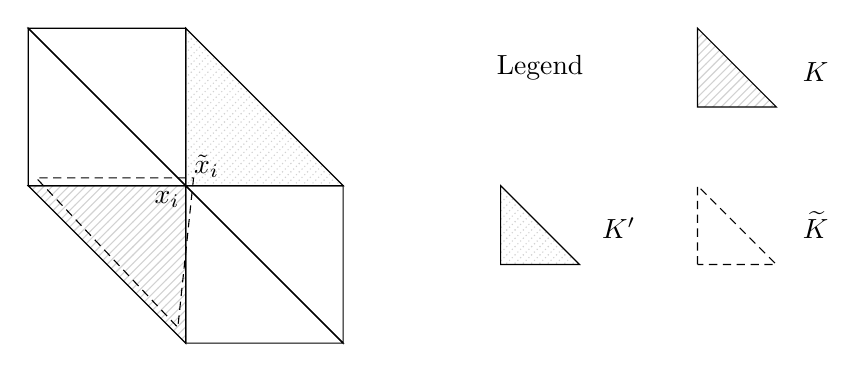
\begin{tikzpicture}
		% Pattern of triangles
		\draw[preaction={clip, postaction={pattern=north east lines, pattern color= {rgb,255:red,210; green,210; blue,210}}}] (2,2) -- (2,0) -- (0,2) -- cycle;
		\draw (2,2) -- (2,0) -- (4,0) -- cycle;
		\draw (2,2) -- (0,2) -- (0,4) -- cycle;
		\draw (2,2) -- (2,4) -- (0,4) -- cycle;
		\draw[preaction={clip, postaction={pattern=north east lines, densely dotted, pattern color= {rgb,255:red,210; green,210; blue,210}}}] (2,2) -- (2,4) -- (4,2) -- cycle;
		\draw (2,2) -- (4,2) -- (4,0) -- cycle;
		% Modified triangles
		\draw[densely dashed] (2.1,2.1) -- (1.9, 0.2) -- (0.1, 2.1) -- cycle;
		% Points
		\node[anchor = north east, inner sep = 2pt] at (2, 2) (xi) {$x_i$}; 
		\node[anchor = south west, inner sep = 0] at (2.1, 2.1) (xitilde) {$\tilde x_i$};
		% Legend
		\node at (6.5, 3.5) (leg) {Legend}; 
		\draw[preaction={clip, postaction={pattern=north east lines, pattern color= {rgb,255:red,210; green,210; blue,210}}}] (8.5,3) -- (8.5,4) -- (9.5,3) -- cycle;
		\node at (10,3.5) (legK) {$\vphantom{\btilde K}K$};
		\draw[preaction={clip, postaction={pattern=north east lines, densely dotted, pattern color= {rgb,255:red,210; green,210; blue,210}}}] (6,1) -- (6,2) -- (7,1) -- cycle;
		\node at (7.5,1.5) (legK2) {$\vphantom{\btilde K} K'$};
		\draw[densely dashed] (8.5,1) -- (8.5,2) -- (9.5,1) -- cycle;
		\node at (10,1.5) (legKtilde) {$\btilde K$};
	\end{tikzpicture}
	\caption{Scheme for error analysis.}
	\label{fig:Error2D}
\end{figure}

Establish \cref{lem:Interp1D} in the two-dimensional case

\begin{lemma}\label{lem:Interp2D} \corr{Restate \cref{lem:Interp1D} in the 2d case.}
\end{lemma}
\begin{proof} Let us denote $e_h = \btilde \Pi_h v_h - v_h$. By definition $e_h(\tilde x_i) = 0$ for all $i = 0, \ldots, N$ and thanks to \cref{lem:InterpPreliminary}
	\begin{equation}\label{eq:ValueNodes}
		e_h(x_i) = h^p \alpha_i \big(\nabla v_h(\tilde x_i) - \nabla \btilde \Pi_hv_h(x_i)\big).
	\end{equation}
	In the following, we denote by $\epl_i$ the quantity
	\begin{equation}
		\epl_i = \nabla v_h(\tilde x_i) - \nabla \btilde \Pi_h v_h(x_i).
	\end{equation}
	Before proceeding to the actual estimation of the error, we shall now bound $\abs{\epl_i}$. Let us denote by $K$ an arbitrary element which has $x_i$ as a vertex and such that the corresponding element $\btilde K$ in the perturbed mesh contains $x_i$. Furthermore, let us denote by $K'$ the element in the original mesh containing $\tilde x_i$. We refer to \cref{fig:Error2D} for a schematic representation of these elements. With this notation, we have $\nabla v_h(\tilde x_i) = \nabla v_h\eval{K'}$, $\nabla \btilde \Pi_hv_h(x_i) = \nabla \btilde \Pi_h v_h\eval{\btilde K}$, and we can then decompose $\epl_i$ in two terms $\epl_{i, 1}$ and $\epl_{i, 2}$, defined as
	\begin{equation}
	\begin{aligned}
		\epl_{i, 1} &= \nabla v_h\eval{K'} - \nabla v_h\eval{K}, \\
		\epl_{i, 2} &= \nabla v_h\eval{K}  - \nabla \btilde \Pi_h v_h \eval{\btilde K},
	\end{aligned}	
	\end{equation}
	so that $\abs{\epl_i} \leq \abs{\epl_{i, 1}} + \abs{\epl_{i, 2}}$. Thanks to \cref{thm:CiarletUniform} we have
	\begin{equation}\label{eq:gradDiffSmooth2d}
	\begin{aligned}
	\abs{\epl_{i, 1}} &\leq 2 \abs{v_h - v}_{\WW^{1,\infty}(D)} + \abs{\nabla v(\bar x_K) - \nabla v(\bar x_{K'})}\\
	&\leq C h \abs{\log h} \abs{v}_{\WW^{2, \infty}(D)},
	\end{aligned}
	\end{equation}
	where we denote by $\bar x_K$ the barycenter of element $K$. Let us now consider $\epl_{i, 2}$. We denote by $B_K$ and $B_{\btilde K}$ the matrices identifying the affine transformations mapping $K$ and $\btilde K$ to the reference triangle $\bhat K$, with vertices $\hat x_1 = (0, 0)^\top$, $\hat x_2 = (1, 0)^\top$, $\hat x_3 = (0, 1)^\top$. In particular, ordering arbitrarily the vertices of $K$ and $\btilde K$ and calling them $x_i$, $\tilde x_i$, $i = 1, 2, 3$ respectively, we have
	\begin{equation}
	\begin{aligned}
		B_K &= \begin{pmatrix} x_2 - x_1 \mid x_3 - x_1 \end{pmatrix},\\
		B_{\btilde K} &= \begin{pmatrix} \tilde x_2 - \tilde x_1 \mid \tilde x_3 - \tilde x_1\end{pmatrix}\\
		&= B_K + h^p \Lambda,
	\end{aligned}
	\end{equation}
	where
	\begin{equation}
		\Lambda = \begin{pmatrix} \alpha_2 - \alpha_1 \mid \alpha_3 - \alpha_1 \end{pmatrix}.
	\end{equation}
	Then (introduce notations)
	\begin{equation}
		\abs{\nabla v_h\eval{K} - \nabla \btilde \Pi_h v_h \eval{\btilde K}} = \abs{B_K^{-\top}\nabla \bhat{v_h} - B_{\btilde K}^{-\top}\nabla \bhat{\btilde \Pi_h v_h}}.
	\end{equation}
	Thanks to \eqref{eq:TaylorVh} we can write
	\begin{equation}
		\nabla \bhat{\btilde \Pi_h v_h} = \nabla \bhat{v_h} + h^p \gamma, 
	\end{equation}
	where the vector $\gamma$ is given by
	\begin{equation}
		\gamma = \begin{pmatrix} \alpha_2^\top \nabla v_h(\tilde x_2) - \alpha_1^\top \nabla v_h(\tilde x_1) \\
		                         \alpha_3^\top \nabla v_h(\tilde x_3) - \alpha_1^\top \nabla v_h(\tilde x_1) \end{pmatrix}.
	\end{equation}
	With algebraic operations we can rewrite $B_{\btilde K}^{-\top}$ as 
	\begin{equation}
	\begin{aligned}
		B_{\btilde K}^{-\top} &= (B_K + h^p \Lambda)^{-\top} \\ 
		&= B_K^{-\top}(I + h^p B_K^{-1}\Lambda)^{-\top} \\
		&= B_K^{-\top}(I - h^p \Gamma),
	\end{aligned}
	\end{equation}
	where the matrix $\Gamma$ is given by the series expansion $\Gamma = \sum_{j=0}^\infty \Gamma_j$, with
	\begin{equation}
		\Gamma_j = (-1)^j h^{pj} (\Lambda^\top B_K^{-\top})^{j+1}.
	\end{equation} 
	Since $\abs{B_K^{-1}} \leq Ch$ \cite[Theorem 3.1.3]{Cia02}, the single addends $\Gamma_j$ satisfy $\abs{\Gamma_j} \leq Ch^{j(p-1)-1}$. Let us remark that the expression above implies $\Gamma_j = -h^p \Gamma_{j-1} \Gamma_0$. Rearranging the terms, we finally get
	\begin{equation}
	\begin{aligned}
		\abs{\nabla v_h\eval{K} - \nabla \btilde \Pi_h v_h \eval{\btilde K}} &= h^p \abs{B_K^{-\top}(-\gamma + \Gamma \nabla \bhat{v_h} + h^p \Gamma \gamma)} \\
		&= h^p \bigg\lvert B_K^{-\top} \Bigl(-\gamma + \Gamma_0 \nabla \bhat{v_h} + \sum_{j=1}^\infty (\Gamma_j\nabla \bhat{v_h} + h^p \Gamma_{j-1} \gamma)\Bigr)\bigg\rvert \\
		&= h^p \bigg\lvert B_K^{-\top} h^p \sum_{j=0}^\infty \Gamma_{j-1} (\gamma -\Gamma_0\nabla \bhat{v_h})\bigg\rvert,
	\end{aligned}
	\end{equation}
	where we define $\Gamma_{-1} = -h^{-p}I$. We can now compute explicitly the difference $\gamma - \Gamma_0 \nabla \bhat{v_h}$ as
	\begin{equation}
	\begin{aligned}
		\gamma - \Gamma_0 \nabla \bhat{v_h} &= \gamma - \Lambda^\top B_K^{-\top} \nabla \bhat{v_h}\\
		&= \gamma - \Lambda^\top \nabla v_h \eval{K} \\
		&= \begin{pmatrix} \alpha_2^\top \nabla v_h(\tilde x_2) - \alpha_1^\top \nabla v_h(\tilde x_1) \\
		\alpha_3^\top \nabla v_h(\tilde x_3) - \alpha_1^\top \nabla v_h(\tilde x_1) \end{pmatrix}
		- \begin{pmatrix} (\alpha_2^\top - \alpha_1^\top) \nabla v_h \eval{K} \\ (\alpha_3^\top - \alpha_1^\top) \nabla v_h \eval{K}	\end{pmatrix}\\
		&= \begin{pmatrix} \alpha_2^\top \big(\nabla v_h(\tilde x_2) - \nabla v_h \eval{K}\big) + \alpha_1^\top \big(\nabla v_h \eval{K} - \nabla v_h(\tilde x_1)\big) \\
						   \alpha_3^\top \big(\nabla v_h(\tilde x_3) - \nabla v_h \eval{K}\big) + \alpha_1^\top \big(\nabla v_h \eval{K} - \nabla v_h(\tilde x_1)\big) \end{pmatrix}.                
	\end{aligned}
	\end{equation}	
	Reasoning as in \eqref{eq:gradDiffSmooth2d} we thus have
	\begin{equation}
		\abs{\gamma - \Gamma_0 \nabla \bhat{v_h}} \leq Ch \abs{\log h}\abs{v}_{\WW^{2, \infty}(D)},
	\end{equation}
	which implies 
	\begin{equation}
		\abs{\nabla v_h\eval{K} - \nabla \btilde \Pi_h v_h \eval{\btilde K}} \leq h^{p+1}\abs{\log h}\abs{v}_{\WW^{2, \infty}(D)} \abs{B_K^{-\top}} \sum_{j=0}^{\infty} h^p \abs{\Gamma_{j-1}}.
	\end{equation}
	From the definition of $\Gamma_j$, $j = -1, 0, \ldots, \infty$, we have $\sum_{j=0}^{\infty} h^p \abs{\Gamma_{j-1}} \leq C$, which finally gives
	\begin{equation}
		\abs{\nabla v_h\eval{K} - \nabla \btilde \Pi_h v_h \eval{\btilde K}} \leq C h^p \abs{\log h} \abs{v}_{\WW^{2, \infty}(D)}.
	\end{equation}
	Since $p \geq 1$, the triangular inequality yields $\epl_{i} \leq Ch \abs{\log h} \abs{v}_{\WW^{2, \infty}(D)}$ for each node. Replacing this bound in \eqref{eq:ValueNodes}, we get for each $x_i \in \mathcal N_h^I$
	\begin{equation}
		\abs{e_h(x_i)} \leq C h^{p+1} \alpha_i \abs{\log h} \abs{v}_{\WW^{2, \infty}(D)}.
	\end{equation}
	Let us now remark that since $e_h \in V_h^+$ and by definition $e_h(\tilde x_i) = 0$ for all modified nodes, the maximum of $e_h$ has to be realised on one of the nodes of the original mesh. Hence
	\begin{equation}
		\norm{e_h}_{\LL^{\infty}(D)} = \max_{x_i \in \mathcal N_h^{I}} \abs{e_h(x_i)} \leq C h^{p+1} \abs{\log h} \abs{v}_{\WW^{2, \infty}(D)},
	\end{equation}
	which implies the desired result for all $\LL^q$ spaces with $1 \leq q < \infty$.
\end{proof}

\section{A probabilistic a posteriori error estimator}\label{sec:errorestimation}
 
Several techniques exist for obtaining a posteriori error estimators in the framework of the FEM (see \cite{Ver13} for an overview), with the twofold goal of controlling the quality of numerical solutions and hence improve the meshing procedure to maximise efficiency. The main purpose of probabilistic numerical methods is to quantify the uncertainty introduced by approximate computations \cite{HOG15}. For the reasons above, we believe that deriving an error estimator from a family of numerical solutions fits perfectly in the probabilistic framework. In this section we present such a procedure for a probabilistic error estimation.
\begin{assumption}\label{as:Saturation} Let $u_h^+ \in V_h^+$ be defined in \eqref{eq:uHPlus}. Then we assume there exists $0 \leq \beta < 1$ such that
	\begin{equation}
		\normm{u - u_h^+} \leq \beta \normm{u - u_h},
	\end{equation} 
	where $\normm{u}^2 = a(u, u)$. Moreover, there exists a constant $\gamma > 0$ such that
	\begin{equation}\label{eq:Saturation2}
		\normm{u_h - u_h^+} \leq \gamma \normm{u_h - \tilde u_h},
	\end{equation}
	almost surely, where $\tilde u_h$ is the probabilistic solution.
\end{assumption}


Let us remark that since $V_h \subset V_h^+$, we have $\beta \leq 1$ for the best approximation property of the Galerkin method and that \cref{as:Saturation} is often denoted in literature as the saturation assumption.

\begin{lemma} Let us denote by $w_h \in V_h$ and $\tilde w_h \in \btilde V_h$ the components of $u_h^+$, i.e., $u_h^+ = w_h + \tilde w_h$. Then
	\begin{equation}
		\abs{w_h(x_i) - \tilde w_h(\tilde x_i)} \leq 
	\end{equation}
	and 
	\begin{equation}
		\normm{w_h - \tilde w_h} \leq
	\end{equation}
\end{lemma}
\begin{proof}

\end{proof}

\begin{lemma} Let us denote by $z_h \in V_h$ the function $z_h = w_h - u_h /2$. Then
	\begin{equation}
		\normm{z_h - \btilde \Pi_h z_h} \leq \ldots
	\end{equation}
\end{lemma}

\begin{proof} 
	\begin{equation}
		\normm{z_h} \leq \frac12 \normm{w_h - \tilde w_h}.
	\end{equation}
\end{proof}

\begin{lemma} Under \ldots, there exists $\gamma > 0$ independent of $h$ and $p$ such that
	\begin{equation}
		\normm{u_h - u_h^+} \leq \gamma \normm{u_h - \tilde u_h},
	\end{equation}
	almost surely in $\Omega$.
\end{lemma}
\begin{proof} Let us write $u_h^+ = w_h + \tilde w_h$, where $w_h$ and $\tilde w_h$ are the two components of $u^+_h$ in $V_h$ and $\btilde V_h$ respectively. For any $v_h^+ \in V_h^+$, $v_h^+ = v_h + \tilde v_h$, with $v_h \in V_h$ and $\tilde v_h \in \btilde V_h$, by Galerkin orthogonality 
	\begin{equation}
	\begin{aligned}
		a(u_h^+ - u_h, v_h^+) &= a(u_h^+ - u_h, \tilde v_h) - a(u_h^+ - \tilde u_h, \tilde v_h) \\
		&= a(\tilde u_h - u_h, \tilde v_h).
	\end{aligned}
	\end{equation}
	Choosing $v_h^+ = u_h^+ - u_h$, we have $\tilde v_h = \tilde w_h$ and 
	\begin{equation}
		\normm{u_h^+ - u_h}^2 = a(\tilde u_h - u_h, \tilde w_h).
	\end{equation}
	The same procedure applied to $u_h^+ - \tilde u_h$ yields
	\begin{equation}
		\normm{u_h^+ - \tilde u_h}^2 = a(u_h - \tilde u_h, w_h).
	\end{equation}
	Hence
	\begin{equation}
		\normm{u_h^+ - u_h}^2 + \normm{u_h^+ - \tilde u_h}^2 = a(u_h - \tilde u_h, w_h - \tilde w_h).
	\end{equation}
	Let us introduce the functions $z_h = w_h - u_h/2 \in V_h$ and $\tilde z_h = \tilde w_h - \tilde u_h /2 \in \btilde V_h$. Then
	\begin{equation}
	\begin{aligned}
		\normm{u_h^+ - u_h}^2 + \normm{u_h^+ - \tilde u_h}^2 &= \frac12 a(u_h - \tilde u_h, u_h - \tilde u_h) + a(u_h - \tilde u_h, w_h - \frac{u_h}{2} - (\tilde w_h - \frac{\tilde u_h}{2}))\\
		&= \frac{1}{2} \normm{u_h - \tilde u_h}^2 + a(u_h - \tilde u_h, z_h - \tilde z_h).
	\end{aligned}
	\end{equation} 
	Consider now the second term in the sum. Adding and subtracting $a(u_h^+, z_h - \tilde z_h)$ and considering Galerkin orthogonality we obtain
	\begin{equation}
		a(u_h - \tilde u_h, z_h - \tilde z_h) = a(u_h - u_h^+, v_h - \tilde z_h) + a(u_h^+ - \tilde u_h, z_h - \tilde v_h),
	\end{equation} 
	for all $v_h \in V_h$ and $\tilde v_h \in \btilde V_h$. Hence, applying Cauchy--Schwarz and Young's inequalities we obtain
	\begin{equation}
		\normm{u_h^+ - u_h}^2 + \normm{u_h^+ - \tilde u_h}^2 \leq \normm{u_h - \tilde u_h}^2 + \inf_{\vphantom{\tilde v_h \in \btilde V_h}v_h \in V_h} \normm{\tilde z_h - v_h}^2 + \inf_{\tilde v_h \in \btilde V_h} \normm{z_h - \tilde v_h}^2.
	\end{equation} 
\end{proof}

Moreover, since the perturbed mesh and the original mesh could switch their roles by changing the sign to the random perturbations, the same assumption as \eqref{eq:Saturation2} should be imposed for the probabilistic solution, i.e.
\begin{equation}
	\normm{\tilde u_h - u_h^+} \leq \btilde \gamma \normm{u_h - \tilde u_h}.
\end{equation}
Applying the triangular inequality, we get
\begin{equation}
\begin{aligned}
	(\gamma + \btilde \gamma) \normm{u_h - \tilde u_h} &\geq \normm{\tilde u_h - u_h^+} + \normm{u_h - u_h^+} \\
	& \geq \normm{u_h - \tilde u_h},
\end{aligned}
\end{equation}
which implies that $(\gamma + \btilde \gamma) \geq 1$. The duality in the roles of deterministic and probabilistic meshes implies that $\gamma$ and $\btilde \gamma$ should be in general approximately equal, at least asymptotically. Hence, the lower bound above guarantees that neither $\gamma$ nor $\btilde \gamma$ should tend to zero with $h\to 0$.

It is known \cite{BaK93} that under \cref{as:Saturation} the estimate
\begin{equation}
	\norm{u_h - u_h^+}_a \leq \norm{u - u_h}_a \leq \frac{1}{1 - \beta} \norm{u_h - u_h^+}_a,
\end{equation}
holds almost surely. The quantity $\norm{u_h - u_h^+}_a$ thus serves as an a posteriori error estimator for the error. However, computations involving the sum space $V_h^+$ are often intractable if the dimension $d > 1$. Hence, we further expand the upper bound thanks to \eqref{eq:Saturation2} as
\begin{equation}\label{eq:ErrorEstimateFinal}
	\normm{u - u_h} \leq \frac{\gamma}{1 - \beta} \normm{u_h - \tilde u_h},
\end{equation}
which means that the difference between the deterministic and the probabilistic solutions can be employed as an a posteriori upper bound for the error.

\begin{remark} Let us remark that the value of $\beta$ is influenced by the choice of $p$ in \cref{as:MeshPerturbation}. Let us consider the limit case of $p \to \infty$. In this case, the spaces $V_h$ and $\tilde V_h$ coincide, and in turn coincide both with $V_h^+$. Hence, the space $V_h^+$ is in the limit not wider than $V_h$ and one expects $\beta \to 1$. We hence postulate that $\beta = \beta(h, p)$ takes the form
	\begin{equation}
		\beta(h, p) = 1 - \beta_1 h^{\beta_2(p-1)},
	\end{equation}
	for some $0 < \beta_1 \leq 1$ and $\beta_2 > 0$. This is motivated by the fact that the two terms in \eqref{eq:ErrorEstimateFinal} converge with the same rate $\OO(h)$ in case $p = 1$ due to a priori error results. Hence, in this case, $\beta(h, 1)$ is independent of $h$ and equals a constant value $\beta$. Conversely, if $p > 1$, one gets on the right hand side a term of order $\OO(h^{\beta_2(1-p)} h^{(p+1)/2})$, bounding a term of order $\OO(h)$ on the left hand side. Hence, we impose
	\begin{equation}
		\beta_2(1-p) + \frac{p+1}{2} \leq 1,
	\end{equation}
	which, since $p > 1$, gives $\beta_2 \geq 1/2$. Numerical experiments confirm the qualitative behaviour of the function $\beta(h, p)$ explained above, and lead to the good working practice of fixing $p = 1$.
\end{remark}

A more robust estimator could be obtained by averaging a family of $M$ probabilistic solutions $\tilde u_h^{(i)}$, $i = 1, \ldots, M$, obtained by $M$ i.i.d. random perturbations of the original mesh. In particular, we have 
\begin{equation}
	\normm{u - u_h}^2 \leq C \E \normm{u_h - \tilde u_h}^2 \eqqcolon C \eta_h^2,
\end{equation}
where we approximate the estimator $\eta_h$ via Monte Carlo sampling as
\begin{equation}
	\eta_h \approx \sqrt{\frac{1}{M} \sum_{i=1}^M \normm{u_h - \tilde u_h^{(i)}}^2}.
\end{equation}
Taking the expectation over several realisations should in practice provide a sharper error estimator, as in case $p = 1$ a good portion of the domain $D$ is explored by the vertices of several realisations of the random mesh. Let us consider for simplicity the case $\kappa \equiv 1$, so that $\normm{u} = \norm{\nabla u}_{L^2(D)}$ for all $u \in H^1_0(D)$. In this case, we have
\begin{equation}
\begin{aligned}
	\eta_h &= \int_{K} \E \abs{\nabla (u_h - \tilde u_h)}^2 \dd x\\
		   &\approx \int_{K} \E \abs{\E (\nabla u_h) - \nabla \tilde u_h}^2 \dd x\\
		   &= \int_K \trace (\Var \nabla u_h) \dd x.
\end{aligned}
\end{equation}   
Hence, following the probabilistic numerics canon, it is possible to interpret the error estimator as an integral measure of the statistical dispersion of numerical solutions over the domain.

We now consider the task of adapting the mesh. Given the error estimator derived above and a prescribed tolerance, we apply a standard technique for generating a sequence of meshes, which we briefly summarise in the following. Let us first split the estimator over the elements of the original mesh as
\begin{equation}
\begin{aligned}
	\eta_h^2 &= \sum_{K\in \mathcal T_h} \E \int_{K} \kappa \nabla (u_h - \tilde u_h) \cdot \nabla (u_h - \tilde u_h)\\
	&= \sum_{K \in \mathcal T_h} \eta_K^2,
\end{aligned}
\end{equation}
where we consider $\eta_K$ to be an indicator of the error at a local level. If we impose a tolerance level $\epsilon$ for the error, i.e.,
\begin{equation}
	\normm{u - u_h} \leq \epsilon \normm{u_h},  
\end{equation}	 
we obtain that a sufficient condition is given by 
\begin{equation}
	\eta_K \leq \frac{\epsilon \normm{u_h}}{\sqrt{N}},
\end{equation}
where $N$ is the number of elements in $\mathcal T_h$. Hence, we proceed iteratively by refining the mesh around elements which do not fulfil the error requirement until the required tolerance is attained. Coarsening of elements where the error indicator is small could be as well employed for saving computational power. The algorithm for mesh adaptation is given in \cref{alg:MeshAdaptivity}, where safety factors $\mathrm{fac}_1$ and $\mathrm{fac}_2$ are introduced. 

\begin{algorithm}[t]
	\caption{Probabilistic mesh adaptivity.}
	\label{alg:MeshAdaptivity}
	\KwData{$\mathcal T_h^{(0)}$, tolerance $\epl$, safety factors $\mathrm{fac}_1$, $\mathrm{fac}_2$, $M \in \N$.}
	Set $i = 0$ \;
	\While{$\eta_h > \epsilon \normm{u_h} $}{
		Compute $u_h$ and $\normm{u_h}$ \;
		Draw $M$ random meshes and compute $\tilde u_h^{(j)}$ for $j = 1, \ldots, M$ \;
		\For{$K \in \mathcal T_h^{(i)}$}{
			Compute $\eta_K$ \;
			\uIf{$\eta_K > \mathrm{fac}_1 \, \epsilon \normm{u_h} /\sqrt{N}$} {
				Mark element $K$ for refinement \;
			} \ElseIf{$\eta_K < \mathrm{fac}_2 \, \epsilon \normm{u_h} /\sqrt{N}$} {
				Mark element $K$ for coarsening \;
			}
		}
		Build $\mathcal T^{(i+1)}$ \;
		Set $i \leftarrow i + 1$ \;
	}
\end{algorithm}

\section{Inverse problems}\label{sec:inverseproblems}

Probabilistic numerical methods are particularly helpful when inserted in the framework of Bayesian inverse problems (BIPs) involving differential equations, as studied in \cite{AbG18, CGS17} for ODEs, and in \cite{COS17, CCC16} for PDEs. Furthermore, in \cite{LST18} a theoretical basis is laid for ensuring the well-posedness of probabilistic solutions to BIPs.

We consider the framework introduced in \cite{Stu10} and expanded in \cite{DaS11}. With the notation of \eqref{eq:ellipticEquation}, we consider the PDE
\begin{equation}\label{eq:ellipticInverse}
\begin{aligned}
	-\nabla \cdot (\exp(\theta) \nabla u) &= f, &&\text{in } D,\\
	u &= 0, &&\text{on } \partial D,
\end{aligned}
\end{equation}
where the conductivity field $\kappa$ is transformed through an exponential function $\kappa = \exp(\theta)$ in order to ensure positivity and hence well-posedness of the solution. Moreover, we suppose that $u \in \WW^{2, \infty}(D)$ and we let $\mathcal U = \mathrm{add space}$ be the space of admissible log-conductivity fields $\theta$. The BIP consists in retrieving the true value $\theta^\dagger$ of the field $\theta$ given prior information and corrupted observations $z \in \R^m$ given by
\begin{equation}
	z = \mathcal G(\theta^\dagger) + \epl,
\end{equation}
where we assume that $\epl \sim \mathcal N(0, \Sigma_\epl)$ is a Gaussian source of additive noise and $\mathcal G \colon \mathcal U \to \R^m$ is the forward operator. In particular, we can write $\mathcal G = \mathcal O \circ \mathcal S$, where $\mathcal S \colon \mathcal U  \to \WW^{2, \infty}(D)$ is the solution operator, mapping any value of the field $\theta$ to the solution $u$ of \eqref{eq:ellipticInverse}, and $\mathcal O \colon \WW^{2, \infty}(D) \to \R^m$ is the observation operator. In this work, we simply consider $\mathcal O$ to be defined by point-wise evaluations of the solution, i.e., 
\begin{equation}
\mathcal O\colon \theta \mapsto \begin{pmatrix} u(x_1) & u(x_2) & \ldots & u(x_m) \end{pmatrix}^\top.
\end{equation} 
If the prior information is encoded by a prior measure $\mu_0$ over the space $\mathcal U$, then the solution of the BIP is given by the posterior distribution $\mu$ such that its Radon--Nikodym derivative satisfies
\begin{equation}
	\frac{\dd \mu}{\dd \mu_0}(\theta; z) = \frac{1}{Z}\exp(-\Phi(\theta; z)),
\end{equation}
where $\Phi \colon (\LL^{\infty})^d \times \R^m \to \R$ is referred to as the potential function and $Z$ is a normalisation constant. Under the Gaussian assumption for the noise, we have
\begin{equation}
	\Phi(\theta; z) = \frac{1}{2} \norm{z - \mathcal G(\theta)}_{\Sigma_\epl}^2,
\end{equation} 
where the norm $\norm{\cdot}_{\Sigma_\epl}$ is defined as
\begin{equation}
	\norm{y}_{\Sigma_\epl} = \norm{\Sigma_\epl^{-1/2} y}_{\R^m}.
\end{equation}
In the following, we will consider the observations $z$ to be fixed and hence denote $\mu(\dd \theta) = \mu(\dd \theta; z)$ as well as $\Phi(\theta) = \Phi(\theta; z)$. Let us denote by $\mathcal G_h \colon \mathcal U \to \R^m$ the forward model obtained as $\mathcal G_h = \mathcal O \circ \mathcal S_h$, where $S_h \colon \mathcal U  \to V_h$ is the solution operator given by the linear FEM and we still denote by $\mathcal O$ the restriction of $\mathcal O$ to $V_h$. Denoting by $\Phi_h$ the approximate potential, given by
\begin{equation}\label{eq:ApproxPotential}
	\Phi_h(\theta) = \frac{1}{2} \norm{z - \mathcal G_h(\theta)}_{\Sigma_\epl}^2,
\end{equation} 
we obtain the approximate posterior measure $\mu_h$ as 
\begin{equation}\label{eq:ApproxPosterior}
	\frac{\dd \mu_h}{\dd \mu_0}(\theta) = \frac{1}{Z_h}\exp(-\Phi_h(\theta)),
\end{equation}
where $Z_h$ is the normalisation constant. Stuart proved \cite[Theorem 4.6]{Stu10} that under suitable assumptions $\Hell(\mu_h, \mu) \to 0$ for $h \to 0$, where $\Hell(\cdot, \cdot)$ is the Hellinger distance for probability measures. Hence, assuming an infinite computational budget is available it is possible to compute the posterior measure via approximate computations. This result has then been extended to more general priors than Gaussian \cite{DaS16, Sul17}.

It has been shown empirically that under a fixed computational budget, employing a standard numerical method for the approximation of the solution operator $\mathcal S$ can lead to inaccurate results \cite{AbG18, CGS17, COS17}. In particular, in case the variance $\Sigma_\epl$ of the observational noise is small with respect to the discretisation error, the posterior measure $\mu_h$ will be overconfident and peaked away from the true value of the unknown field. Probabilistic numerical methods can efficiently tackle this overconfidence issue thanks to the uncertainty quantification of numerical errors they naturally introduce. Given the probability space $\Omega$ on which the random variables defining the probabilistic scheme $\alpha_i \colon \Omega \to \R^d$ introduced in \cref{as:MeshPerturbation} are defined, let us denote by $\btilde{\mathcal G}_h \colon \Omega \times \mathcal U \to \R^m$ the random forward model obtained as $\btilde{\mathcal G}_h = \mathcal O \circ \btilde{\mathcal S}_h$, where $\btilde{\mathcal S}_h \colon \Omega \times \mathcal U \to \btilde V_h$ is the solution operator corresponding to the random FEM introduced in this work. Replacing $\mathcal G_h$ with $\btilde{\mathcal G}_h$ in \eqref{eq:ApproxPotential} we get a random potential $\btilde \Phi_h$ and eventually a random posterior measure $\tilde \mu_h$ defined by
\begin{equation}
	\frac{\dd \tilde \mu_h}{\dd \mu_0}(\theta) = \frac{1}{\btilde Z_h}\exp(-\btilde \Phi_h(\theta)),
\end{equation}
where $\btilde Z_h$ is the normalisation constant. In order to obtain an approximation of $\mu$ through $\tilde \mu_h$, we need to take the expectation of the random probabilistic solution, which is viable in two different manners as explained in \cite{LST18}. The first approach is to define the measure $\tilde \mu_h^{\mathrm{fix}} = \E \tilde \mu_h$. Otherwise, one could define a measure $\tilde \mu_h^{\mathrm{var}}$ through
\begin{equation}
	\frac{\dd \tilde \mu_h^{\mathrm{var}}}{\dd \mu_0}(\theta) = \frac{1}{\E \btilde Z_h} \E \exp(-\btilde \Phi_h(\theta)),
\end{equation}
which is already a deterministic measure. The choice of the names of these two approximation comes from their computation, which is in spirit slightly different. In the case of $\tilde \mu_h^{\mathrm{fix}}$, for each event $\omega$ one evaluates the forward model and computes the value of the posterior. The expectation is then taken with the respect to the posterior itself, in practice via averaging techniques. Hence, for each $\omega$ we fix a perturbed mesh $\btilde {\mathcal T}_h(\omega)$ and compute the posterior for several values of $\theta$. Conversely, in the case of the measure $\tilde \mu_h^{\mathrm{var}}$ the field $\theta$ is first fixed, and then the posterior is in practice obtained evaluating the forward model on several (variable) realisations of the random probabilistic solution.

We now need to prove the convergence of the posterior distributions $\tilde \mu_h$ and $\tilde \mu_h^{\mathrm{var}}$ towards the true posterior $\mu$ with respect to the mesh size, which is granted by the following result under three regularity assumptions.
\begin{theorem}[Theorem 3.9 of \cite{LST18}]\label{thm:ConvergencePosteriorGeneral} With the notation above, if
	\begin{enumerate}
		\item\label{it:hypConvPosterior1} there exists $q > 0$ such that $\exp(\Phi) \in L_{\mu_0}^q(\mathcal U)$,
		\item\label{it:hypConvPosterior2} there exists a constant $C > 0$ such that
		\begin{equation}
			\E_{\mu_0} [\btilde \Phi_N] \leq C, \quad \text{almost surely in } \Omega,
		\end{equation}
		\item\label{it:hypConvPosterior3} it holds
		\begin{equation}
			\lim_{h \to 0} \norm{\left(\E\norm{\btilde{\mathcal G}_h - \mathcal G}^2\right)^{1/2}}_{L^s_{\mu_0}(\mathcal U)} = 0,
		\end{equation}
		where $s = 2q / (q-1)$ and $q$ is given in \ref{it:hypConvPosterior1},
	\end{enumerate}
	then 
	\begin{equation}
	\begin{aligned}
		\E\left[\Hell(\mu, \btilde \mu_h)^2\right]^{1/2} &\leq C \norm{\left(\E\norm{\btilde{\mathcal G}_h - \mathcal G}_{\R^m}^4\right)^{1/2}}^{1/2}_{L_{\mu_0}^2(\mathcal U)}, \\
		\Hell(\mu, \btilde \mu_h^{\mathrm{var}}) &\leq C \norm{\E\norm{\btilde{\mathcal G}_h - \mathcal G}_{\R^m}^2}^{1/2}_{L_{\mu_0}^s(\mathcal U)}. 
	\end{aligned}
	\end{equation}
\end{theorem}
Let us remark that for a measure $\mu$ the spaces $L_{\mu}^q(\mathcal U)$ are defined as
\begin{equation}
	L_{\mu}^q(\mathcal U) = \left\{f \colon \mathcal U \to \R : \int_{\mathcal U} f(\theta)^q \, \mu(\dd \theta) < \infty \right\},
\end{equation}
with norm 
\begin{equation}
	\norm{f}_{L_{\mu}^q(\mathcal U)} = \left(\int_{\mathcal U} f(\theta)^q \, \mu(\dd \theta) \right)^{1/q}.
\end{equation}
\cref{thm:ConvergencePosteriorGeneral} gives in a general framework the convergence of posterior measures defined through approximate random forward models  
The following result now guarantees the convergence of the posterior distributions


\section{Numerical experiments}

\subsection{Convergence}

\subsubsection*{One-dimensional case} 

We consider \eqref{eq:ellipticEquation} with $\kappa \equiv 1$ on $D = (0, 1)$ and $f(x) = (x - 1/2)\chi_{(1/2, 1)}(x)$, so that the solution $u$ satisfies \cref{as:regularity}. We verify the result of \cref{thm:Convergence1D} by choosing $p \in \{1, 2, 3\}$ and by varying the mesh size $h$ in the range $[9\cdot 10^{-3}, 0.25]$. Moreover, we compute only one realisation of the random mesh for each couple $\{p, h\}$ as our bound holds almost surely. Results, shown in \cref{fig:Convergence1D}, confirm the validity of the convergence estimates.
\begin{figure}[t]
	\centering
	\begin{tabular}{cc}
		\includegraphics[]{Figures/Convergence1D_H1} & \includegraphics[]{Figures/Convergence1D_L2} \\
	\end{tabular}
	\caption{Convergence rates in the $H^1$ semi-norm and the $L^2$ norm for the one-dimensional Poisson equation.}
	\label{fig:Convergence1D}
\end{figure}

\subsection{Error estimators}

\subsubsection*{One-dimensional example}

Consider
\begin{equation}
\begin{aligned}
	-u'' &= f, &&\text{in } (0,1), \\
	u(0) = u(1) &= 0,
\end{aligned}
\end{equation}
with $f$ chosen such that $u(x) = -\sin(12\pi x) \exp(-100(x-1/2)^2)$ is the true solution. We consider the error estimations of presented in \cref{sec:errorestimation}, both in a local and global manner. Results, displayed in \cref{fig:ErrEst1D_local,fig:ErrEst1D_global} show that the estimates hold in practice for this case. In particular, in \cref{fig:ErrEst1D_global} we can remark that the overall effectivity index $\eta_{\mathcal X}$, defined as
\begin{equation}
	\eta_{\mathcal X} = \frac{\E\norm{u_h - \tilde u_h}_{\mathcal X}}{\norm{u_h - u}_{\mathcal X}},
\end{equation}
with $\mathcal X = H_0^1, L^2$, is in this case close to one for both norms. Errors are estimated employing $M = 10$ realisations of the probabilistic solution and with a Monte Carlo simulation.

\begin{figure}[t]
	\centering
	\begin{tabular}{cc}
		\includegraphics[]{Figures/ErrEst1D_ExSol} & \includegraphics[]{Figures/ErrEst1D_DetVsProb} \\
		\includegraphics[]{Figures/ErrEst1D_ErrCoarse} & \includegraphics[]{Figures/ErrEst1D_ErrFine} \\
	\end{tabular}
	\caption{Error estimation for the 1D problem with two different values of $h$ -- error in each element.}
	\label{fig:ErrEst1D_local}
\end{figure}

\begin{figure}[t]
	\centering
	\begin{tabular}{cc}
		\includegraphics[]{Figures/ErrEst1D_ConvL2} & \includegraphics[]{Figures/ErrEst1D_EffectL2} \\
		\includegraphics[]{Figures/ErrEst1D_ConvH1} & \includegraphics[]{Figures/ErrEst1D_EffectH1} \\
	\end{tabular}
	\caption{Error estimation for the 1D problem with two different values of $h$ -- convergence of error estimators and effectivity indices}
	\label{fig:ErrEst1D_global}
\end{figure}

\subsubsection*{Two-dimensional case}

\todo

\subsection{Mesh adaptivity}

\subsubsection*{Two-dimensional case}

See results \cref{fig:MeshAdaptivity2D}.

\begin{figure}[t]
	\centering
	\begin{tabular}{cc}
		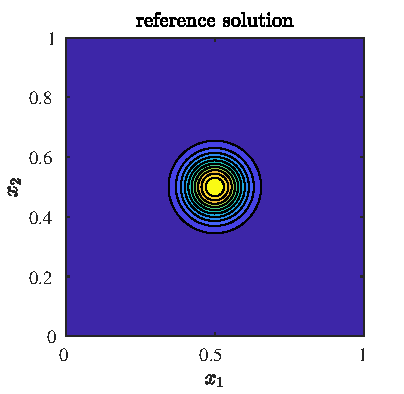
\includegraphics[]{Figures/MeshAdapt2D_ReferenceSol} & 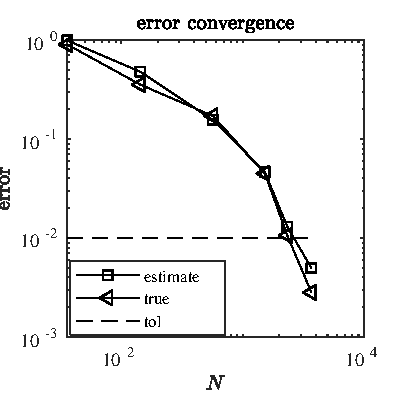
\includegraphics[]{Figures/MeshAdapt2D_ErrConv} \\
		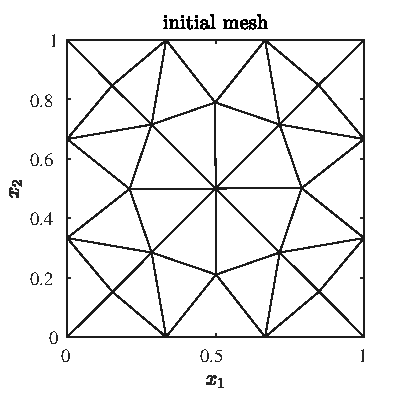
\includegraphics[]{Figures/MeshAdapt2D_InitMesh} & 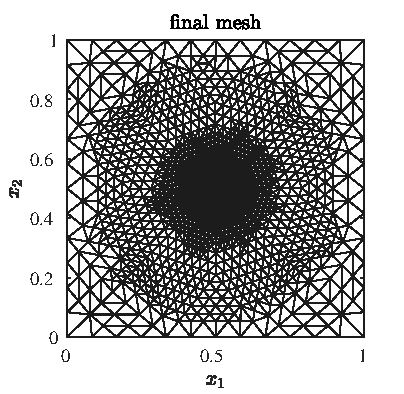
\includegraphics[]{Figures/MeshAdapt2D_FinalMesh}\\
%		\includegraphics[]{Figures/MeshAdapt2D_2_ErrEst} &\includegraphics[]{Figures/MeshAdapt2D_2_TrueErr} \\
	\end{tabular}
	\caption{Mesh adaptivity -- two-dimensional case}
	\label{fig:MeshAdaptivity2D}
\end{figure}

\begin{figure}[t]
	\centering
	\begin{tabular}{cc}
		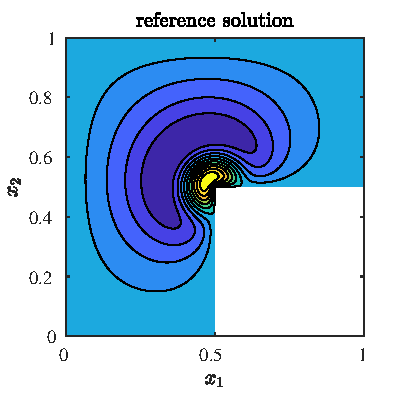
\includegraphics[]{Figures/MeshAdapt2D_2_ReferenceSol} & 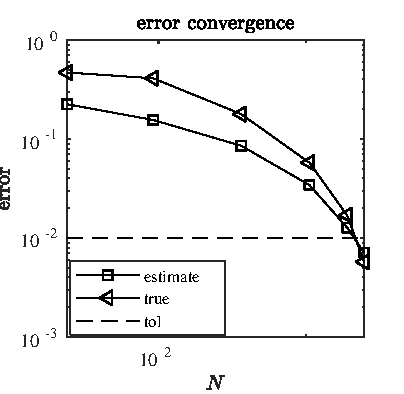
\includegraphics[]{Figures/MeshAdapt2D_2_ErrConv} \\
		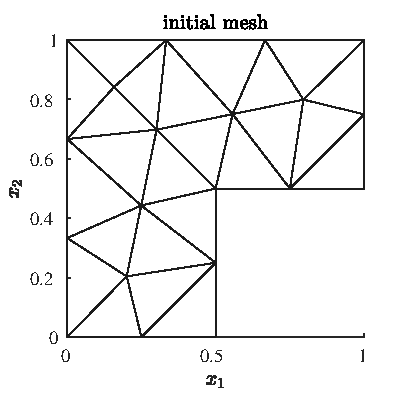
\includegraphics[]{Figures/MeshAdapt2D_2_InitMesh} & 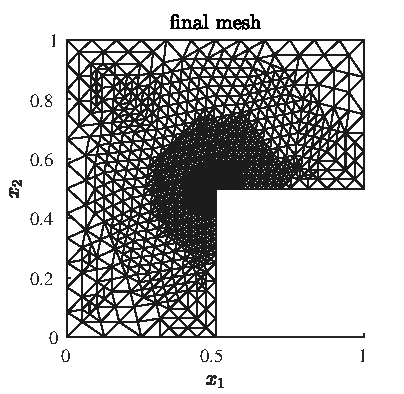
\includegraphics[]{Figures/MeshAdapt2D_2_FinalMesh}\\
%		\includegraphics[]{Figures/MeshAdapt2D_2_ErrEst} &\includegraphics[]{Figures/MeshAdapt2D_2_TrueErr} \\
	\end{tabular}
	\caption{Mesh adaptivity -- two-dimensional case}
	\label{fig:MeshAdaptivity2D_2}
\end{figure}

\subsection{Bayesian inverse problems}

Let us consider the following one-dimensional elliptic equation
\begin{equation}
\begin{aligned}
	-\frac{\dd}{\dd x}\big(e^{\kappa} \frac{\dd u}{\dd x}\big) &= f, &&\text{in } (0,1),\\
	u &= 0, &&\text{on } \{0, 1\},
\end{aligned}
\end{equation}
and the inverse problem of retrieving the field $\kappa \in \LL^2(0, 1)$ given synthetic noisy observations of the solution $u$ corresponding to a true field $\kappa^*$. First, we consider a case where information on $\kappa$ is available beforehand. In particular, we assume that $\kappa$ has the form
\begin{equation}\label{eq:fieldInfo}
	\kappa(x) = \begin{cases}	
				\log(1 + \kappa_1), & \mbox{if } x \in I_1, \\
				\log(1 + \kappa_2), & \mbox{if } x \in I_2, \\	
				0 & \mbox{otherwise},
				\end{cases}
\end{equation}
where $\kappa_1$, $\kappa_2$ are real scalars and $I_1$, $I_2$ are the intervals $(0.2, 0.4)$ and $(0.6, 0.8)$ respectively. Fixing a standard Gaussian prior on both parameters $\kappa_1$ and $\kappa_2$ we are able to compute the posterior distribution corresponding to both the deterministic and probabilistic forward models. In particular, we vary the number of elements $N$ in the set $\{20, 40, 80, 160\}$, thus studying the effects of numerical errors on the numerical posterior distribution. Observations are obtained from a reference solution evaluated at four equispaced points in the interior of $(0, 1)$ each corrupted by an additive source of noise $\epl \sim \mathcal N(0, 10^{-4})$. The posterior distributions are obtained with Metropolis--Hastings initialised near the true value of $(\kappa_1, \kappa_2)$ and ran as explained in \cref{sec:inverseproblems}, with 200 parallel chains employed for the probabilistic forward model. Results are shown in \cref{fig:BayesFin}, where \todo

In a second experiment, we consider the same exact field $\kappa^*$ and observation model, but without the additional information encoded in \eqref{eq:fieldInfo}.

\begin{figure}[t]
	\centering
	\begin{tabular}{cc}
		\includegraphics[]{Figures/Bayes_Fin_Det} & \includegraphics[]{Figures/Bayes_Fin_Prob} \\
	\end{tabular}
	\caption{Bayesian inverse problem -- finite dimensional case.}
	\label{fig:BayesFin}
\end{figure}


%\subsubsection*{L-shaped domain}
%We solve
%\begin{equation}
%\begin{aligned}
%	-\nabla \cdot (\kappa \nabla u) &= f, &&\text{in } D,\\
%	u &= 0, &&\text{on } \delta D,
%\end{aligned}
%\end{equation}
%where $D = (0, 1)^2$ domain and where $\kappa$ is given by
%\begin{equation}
%	\kappa(x) = \begin{cases} 0.1 &\mbox{if } x \in D_1,\\
%	 						  2.5 &\mbox{if } x \in D_2,\\
%	 						  1.3 &\mbox{otherwise},	
%				\end{cases}
%\end{equation}
%where $D_1$ and $D_2$ are the circles with radius $\sqrt{0.025}$ centred in $(0.25, 0.25)$ and $(0.75, 0.75)$


\bibliographystyle{siamplain}
\bibliography{anmc}
\end{document}